\section{Background}

\subsection{Next-Gen G-Wave Astronomy}
\frame{
\frametitle{Next-Generation Gravitational Wave Astronomy}

\begin{columns}
  \begin{column}{.48\textwidth}
    Detector network by $\approx 2020$
    \begin{itemize}
\scriptsize 
    \item[\blacksquare]aLIGO (Washington State)
    \item[\blacksquare]aLIGO (Louisiana)
    \item[\blacksquare]aVIRGO (Italy)
    \item[\blacksquare]GEO-HF (Germany)
    \item[\blacksquare]KAGRA (Japan)
    \item[\blacksquare]LIGO-India
    \end{itemize}
\vspace{1cm}
Candidate Systems
\begin{itemize}
\scriptsize 
\item[\blacksquare]\scriptsize Binary Neutron Star (NS-NS)
\item[\blacksquare]\scriptsize Binary Black Holes (BH-BH)
\item[\blacksquare]\scriptsize Neutron Star - Black Hole (NS-BH)
\end{itemize}

  \end{column}
  \begin{column}{.48\textwidth}
\centering{\text{\tiny [Sathyaprakash
 2014]}}
   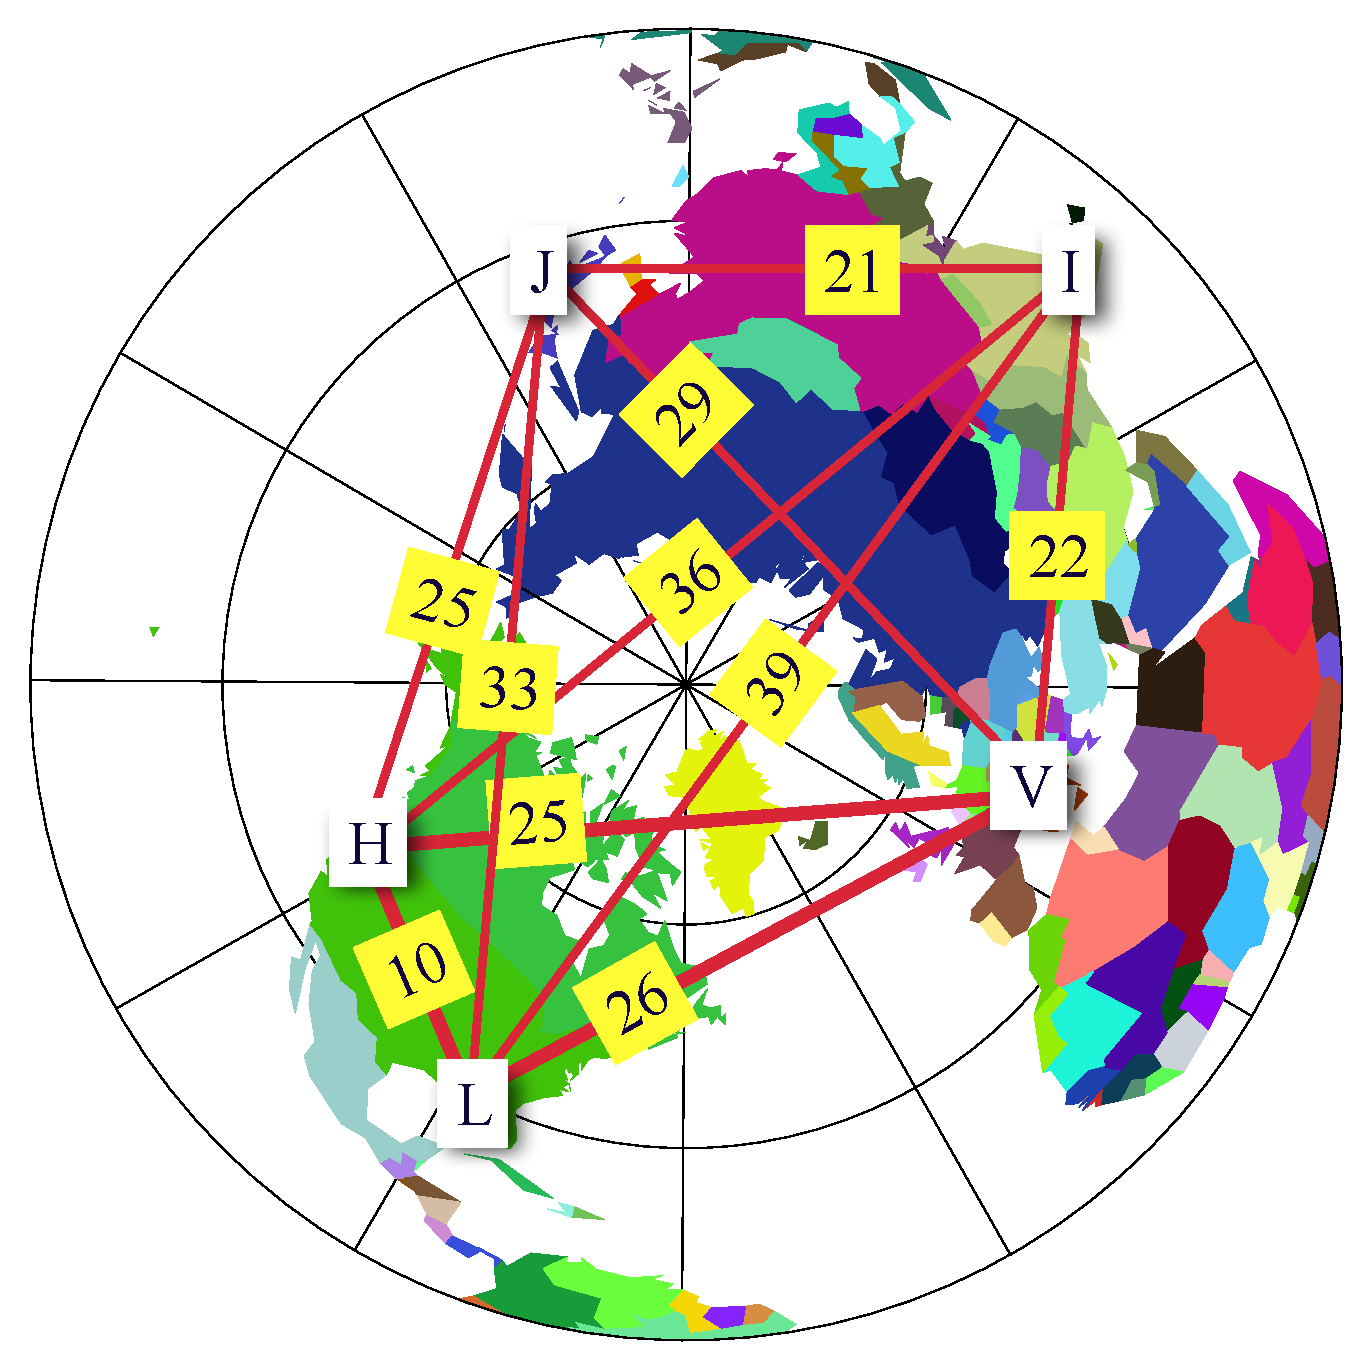
\includegraphics[width=.9\textwidth]{pictures/worldwide.pdf} \\
   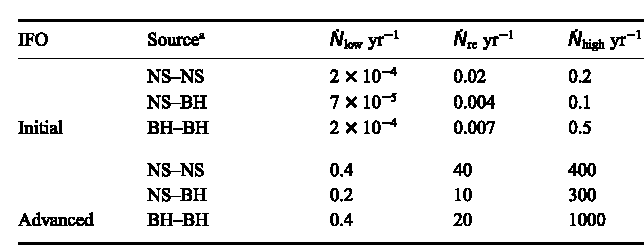
\includegraphics[width=\textwidth]{pictures/abadie.pdf} \\
    \centering{\text{ \tiny [Abadie et al; 1003.2480]}}
  \end{column}
\end{columns}
}

\frame{
\frametitle{Binary Mergers}
\vspace{0cm}
\hspace{0cm}

\includegraphics[width=\textwidth]{pictures/shibata_cropped.pdf}\\
{\tiny Slide adapted from Shibata talk in 2011.}
}

\subsection{Constraining the NS EOS}
\frame{
\frametitle{Neutron Star Equation Of State (EOS)}

\begin{columns}
  \begin{column}{.48\textwidth}
\scriptsize {\boldmath$\text{EOS} \equiv P=P(\rho,T,Y_{e},..)$ still unknown.}\\
\vspace{.6cm}
   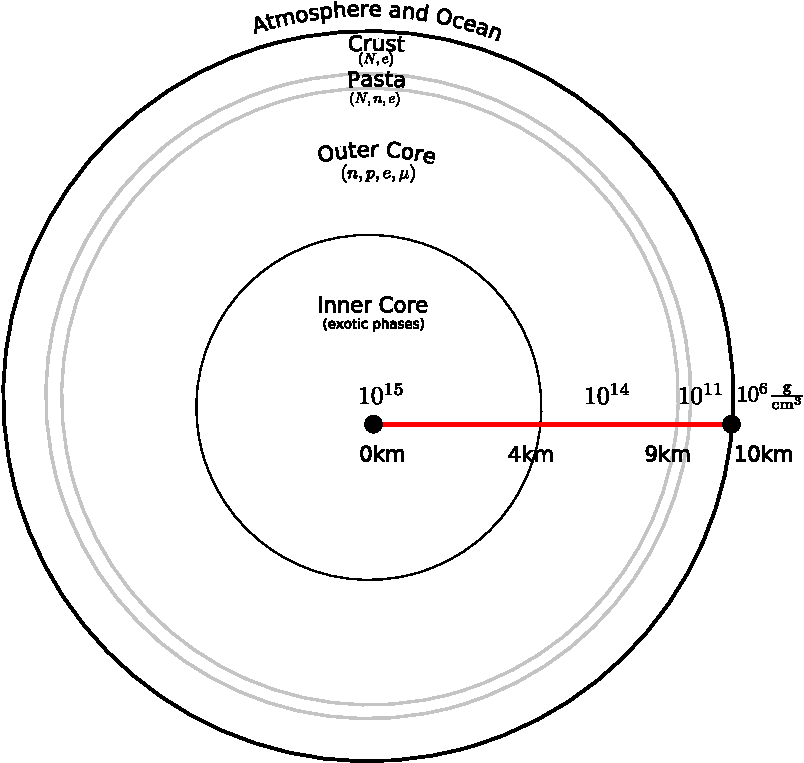
\includegraphics[width=\textwidth]{pictures/ns-crop.pdf} \\
\scriptsize {\vspace{.5cm}A realistic EOS captures microphysics in all theoretical regions.}\\

  \end{column}

  \begin{column}{.48\textwidth}

    \centering \tiny [Lattimer;1305.3510]
\vspace{.05cm}
\centering{ 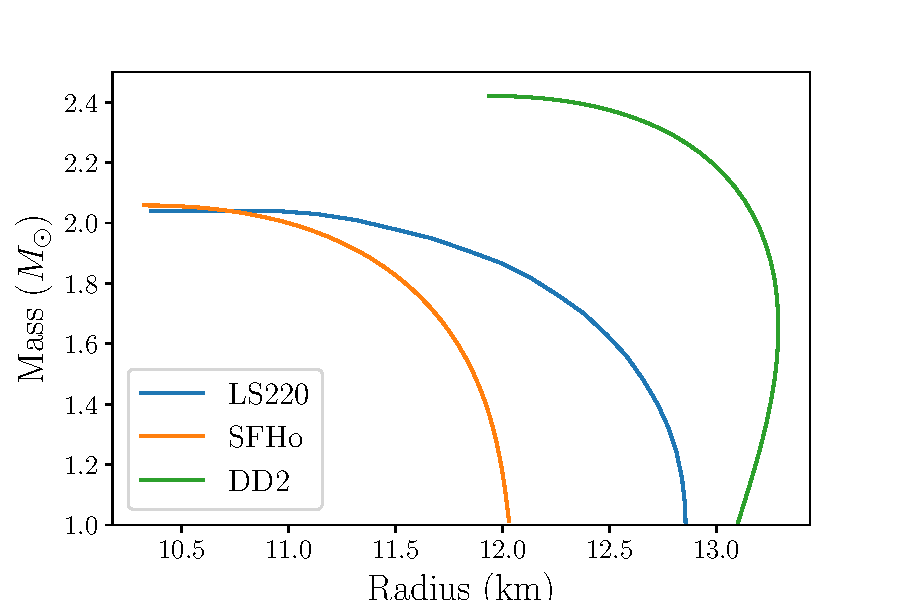
\includegraphics[width=.7\textwidth]{pictures/eos.pdf}} \\


\begin{mybox}{white}{\centering \scriptsize Spherical TOV Star}
\vspace{-.3cm}
\tiny    \begin{equation*}
      \label{eq:1}
      \begin{split}
        &\frac{dP}{dr} = -\frac{(G(m(r)) + 4\pi r^{3}P/c^{2})(\rho + P/c^{2})}{r(r-2Gm(r)/c^{2})} \\
& \frac{dm}{dr} = 4\pi\rho \\
&P = P(\rho, T, Y_{e}, ...)
      \end{split}
    \end{equation*}   
\end{mybox}
  \end{column}
\end{columns}
}

% \frame{
% \frametitle{Constraining the Equation Of State}

% \centering{
% 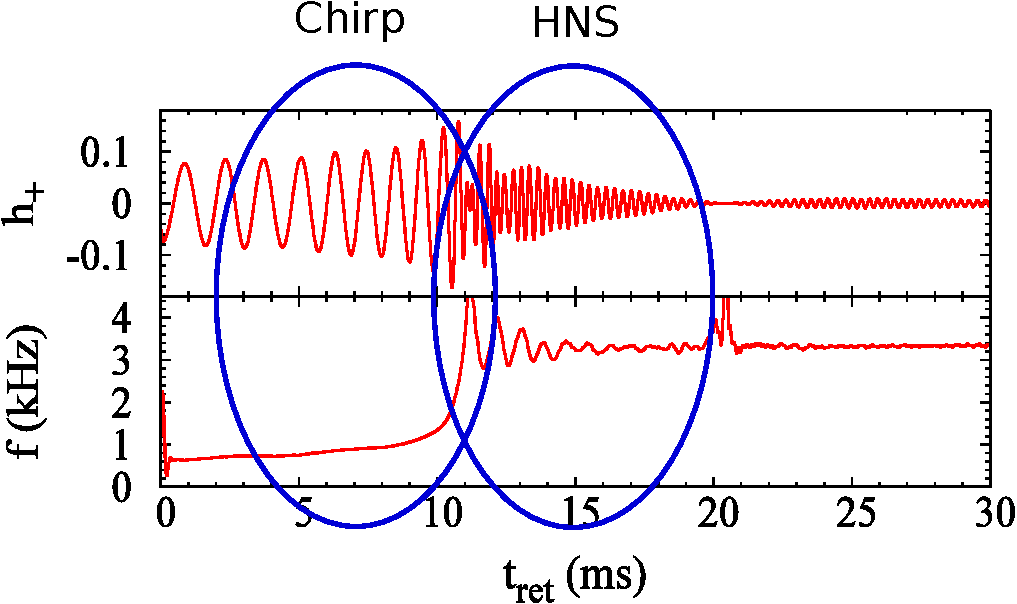
\includegraphics[width=.4\textwidth]{pictures/shibata2.pdf} \\
% }

% % \begin{minipage}
% \begin{columns}

%   \begin{column}{.3\textwidth}
% \vspace{-4cm}
% \centering {   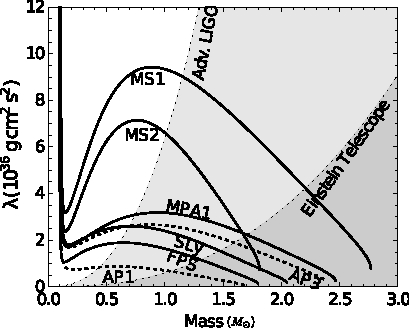
\includegraphics[width=\textwidth]{pictures/lambda.pdf}}
%   \end{column}
%   \begin{column}{.6\textwidth}
% \centering    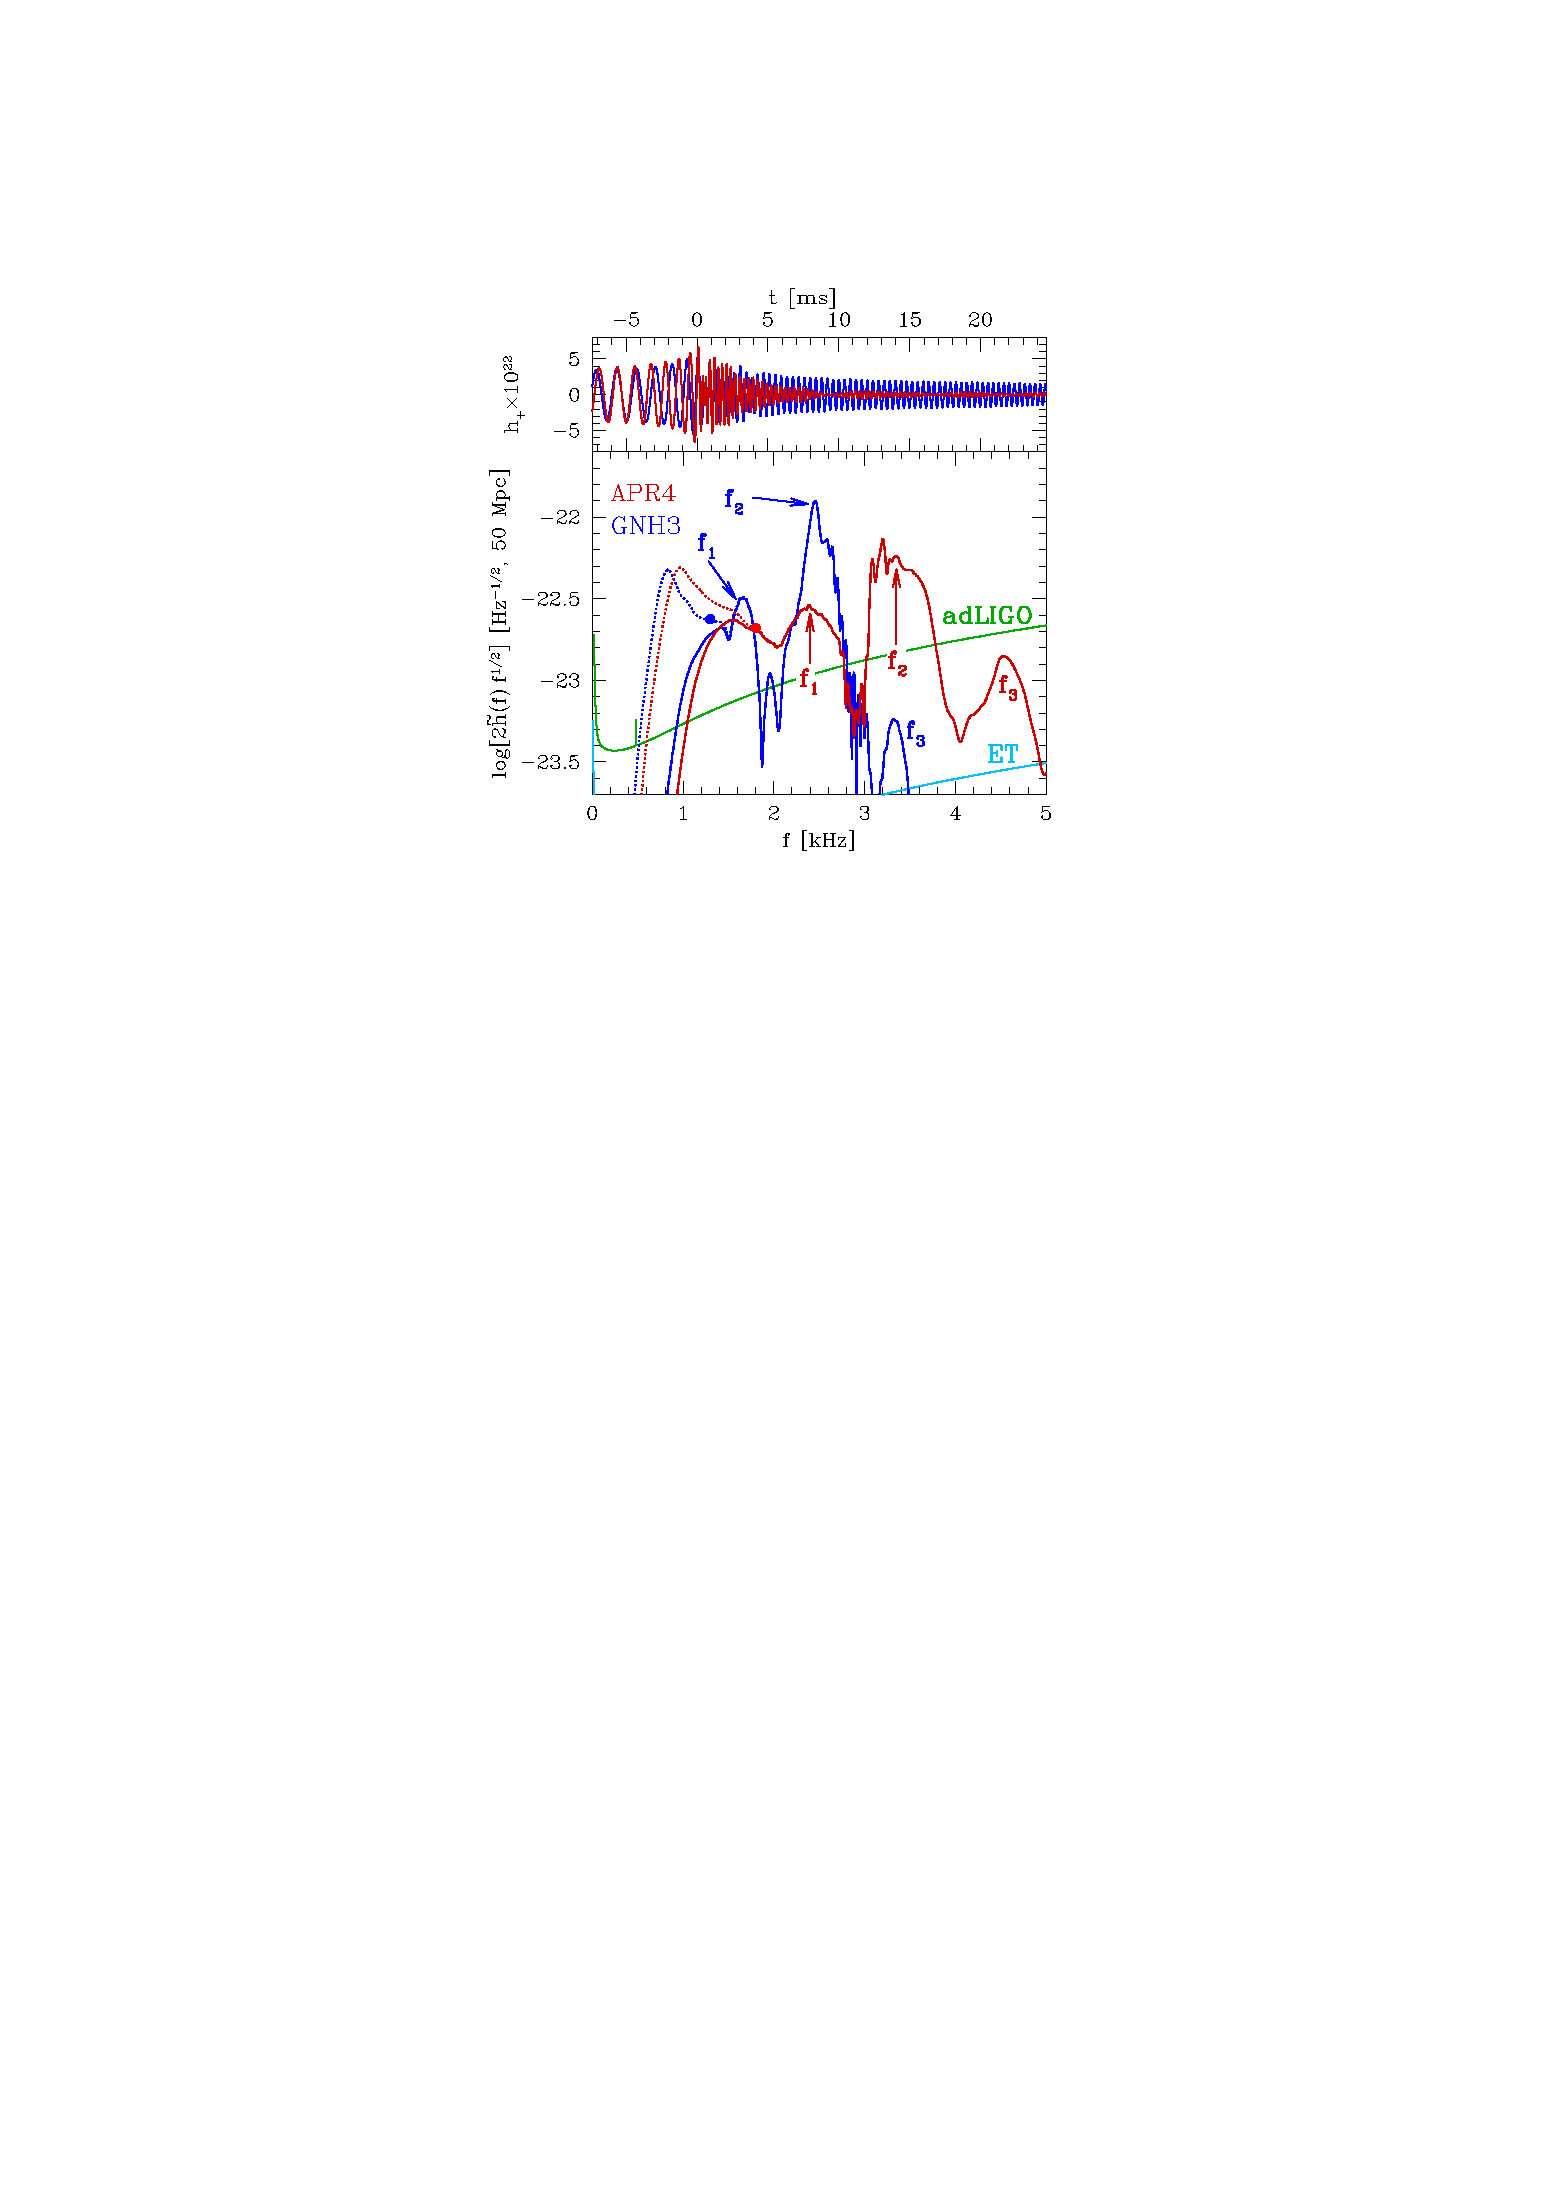
\includegraphics[width=\textwidth]{pictures/f3.pdf} \\
%   \end{column}
% \end{columns}
% % \end{minipage}


% }


\begin{frame}
\frametitle{Constraining the Equation Of State Using GWs}
\begin{columns}
\column{0.5\textwidth}
\begin{minipage}[c][0.4\textheight][c]{\linewidth}
  \centering
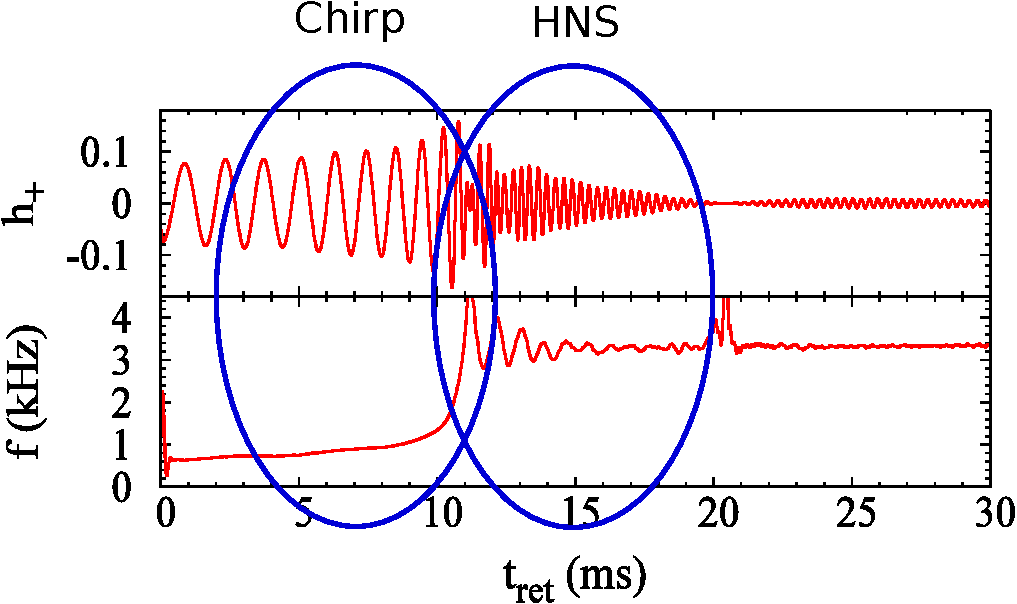
\includegraphics[width=\textwidth]{pictures/shibata2.pdf}
\end{minipage}
\begin{minipage}[c][0.4\textheight][c]{\linewidth}
  \centering
 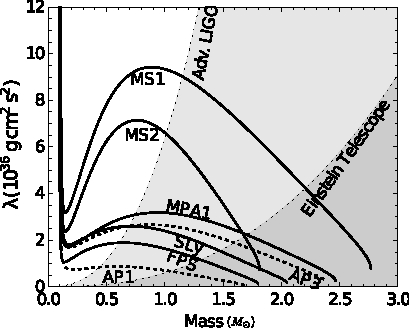
\includegraphics[width=.8\textwidth]{pictures/lambda.pdf}\\
{\tiny [Hinderer et al; 0911.3535]}
\end{minipage}
\column{0.5\textwidth}
\begin{minipage}[c][0.4\textheight][c]{\linewidth}
  \centering{\item[\blacksquare]\textbf{Two Interesting Phases.}}
  \begin{enumerate}
  \item[\blacksquare]Late Inspiral - Tidal Deformability $\lambda$
  \item[\blacksquare]Postmerger HNS - 3 peak frequencies
  \end{enumerate}
\end{minipage}
\begin{minipage}[c][0.4\textheight][c]{\linewidth}
  \centering
  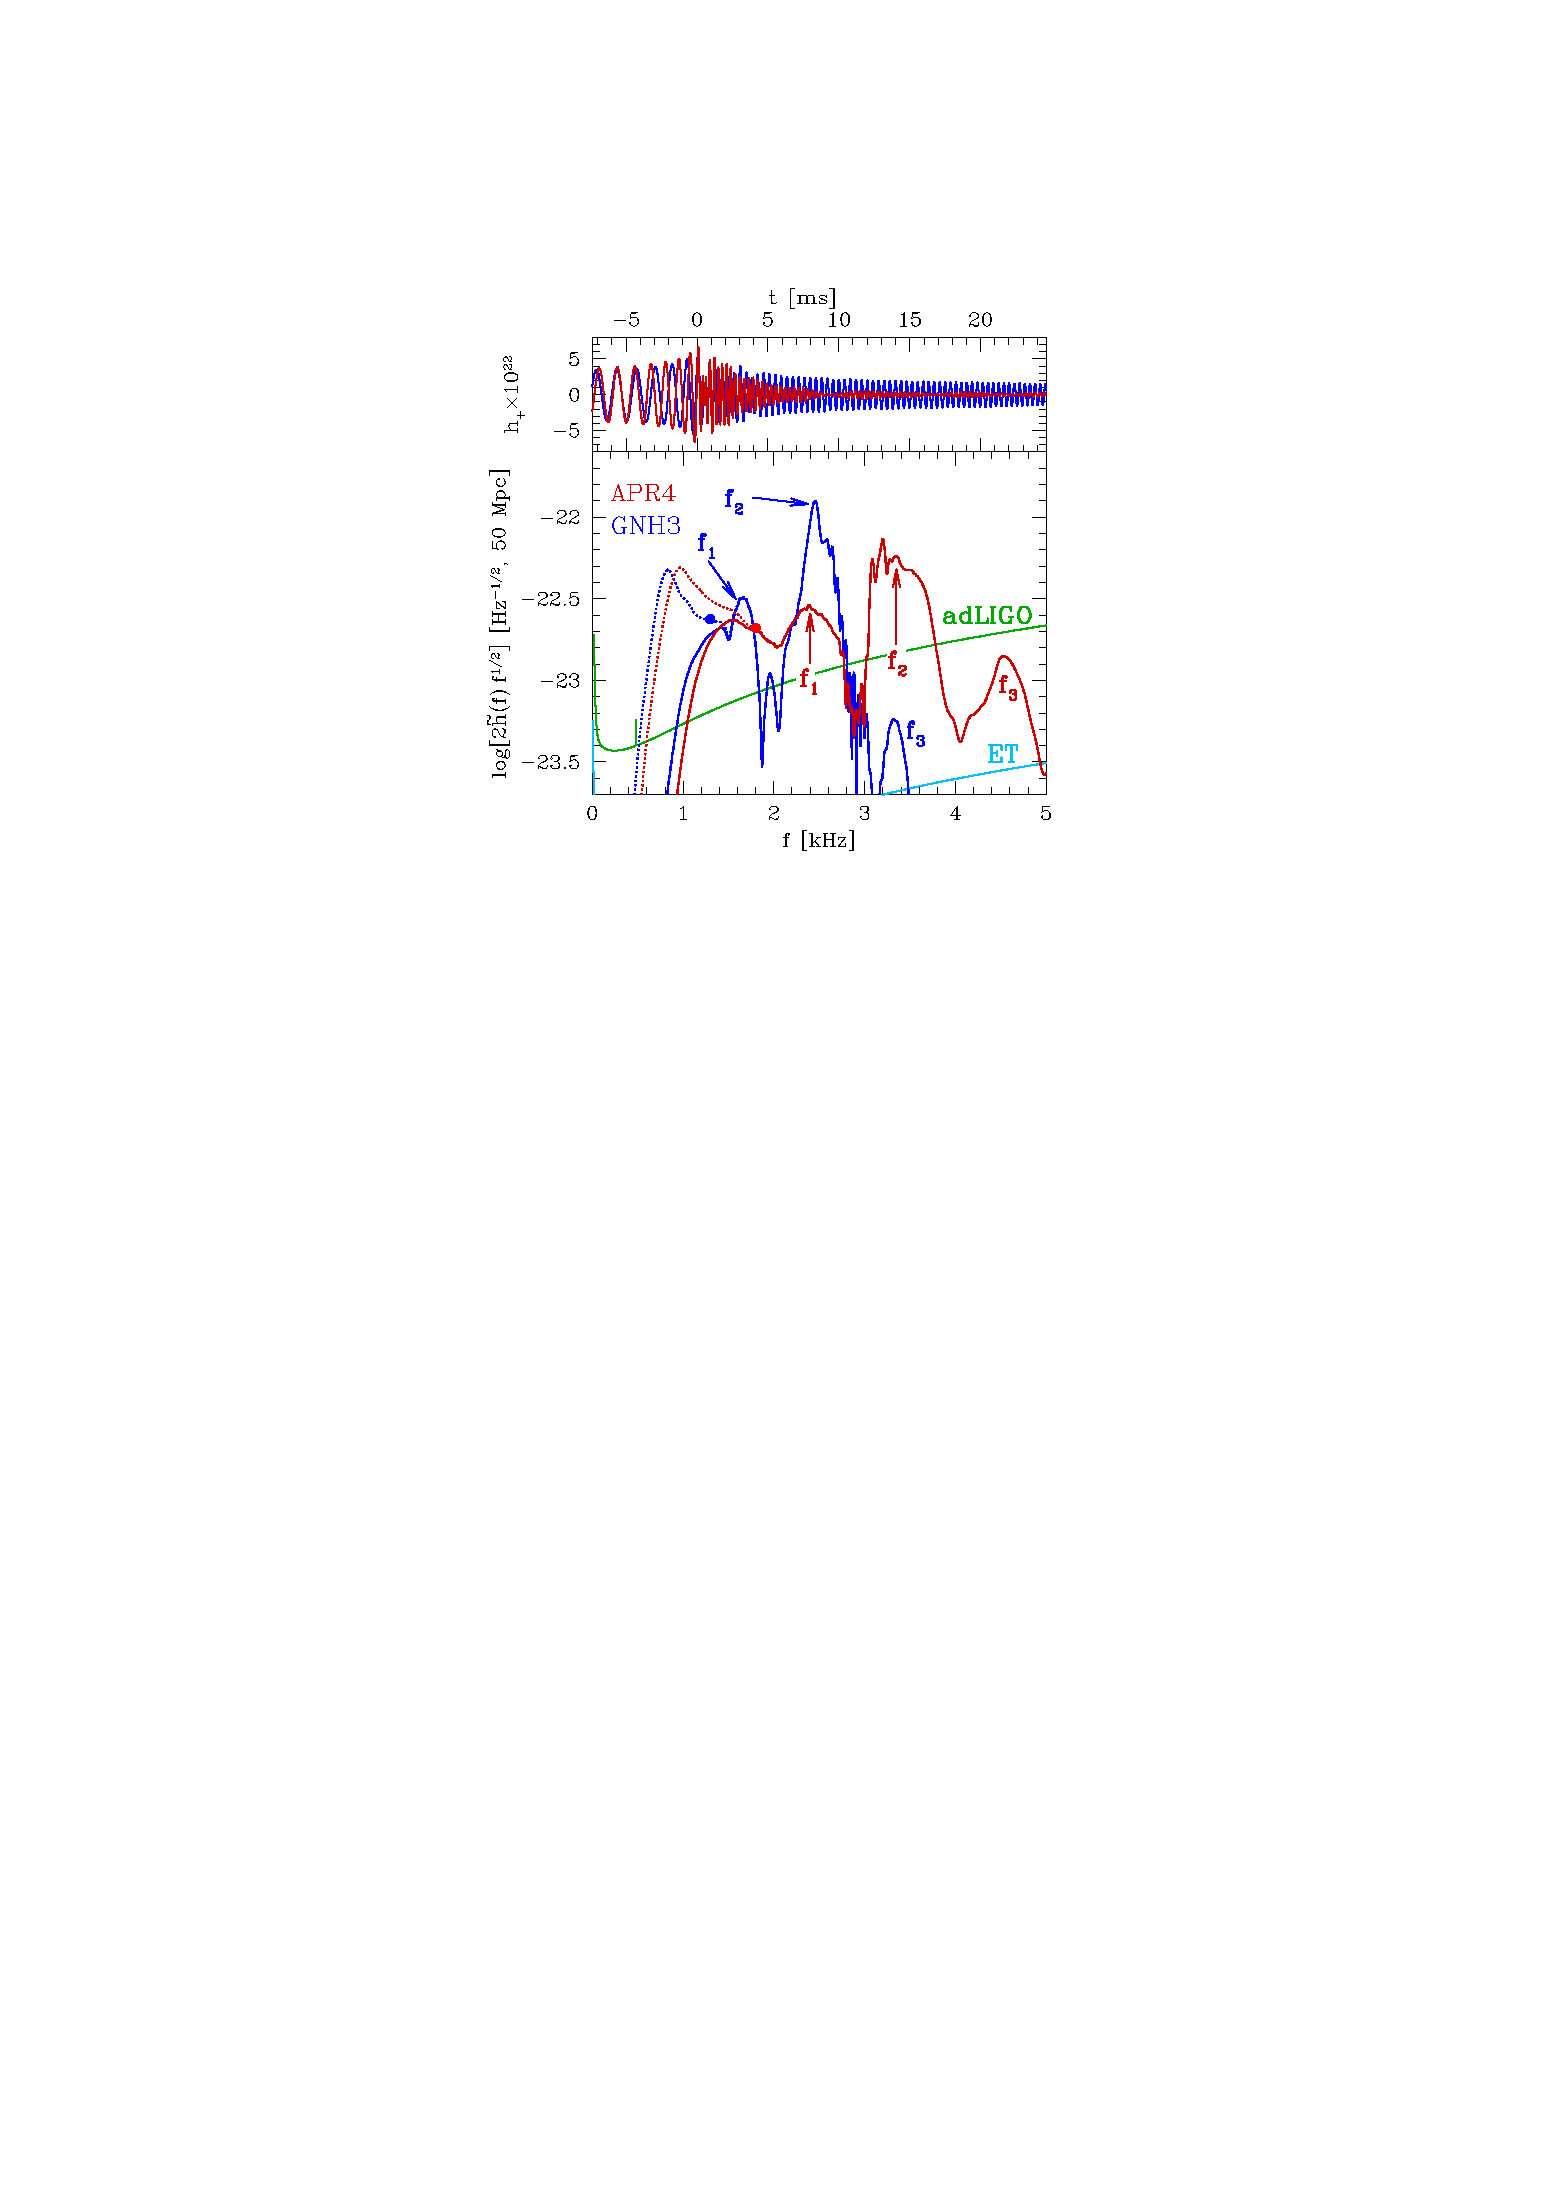
\includegraphics[width=.7\textwidth]{pictures/f3.pdf}\\
\vspace{-.2cm}
{\tiny [Takami et al; 1412.3240]}
\end{minipage}
\end{columns}
\end{frame}

\subsection{SpECTRE: Next-Gen Numerical Relativity}

\frame{
\frametitle{Solving the Field Equations on a Computer}

Write Einstein's field equations as an initial-value problem for $g_{\mu\nu}$\\
\vspace{.5cm}
\begin{mybox}{white}{}
\begin{equation*}
\label{eq:3}
\vspace{.3cm}
\scriptsize
G_{\mu\nu} = 8\pi T_{\mu\nu} \rightarrow \begin{cases}
    \text{Constraints} &  (\text{like  } \nabla \cdot B = 0)\\
    \text{Evolution Equations} & (\text{like  } \partial_{t} B = -\nabla \times E)
\end{cases}
\end{equation*}
\end{mybox} 
\vspace{.3cm}
Obtain a computer cluster and \\
\vspace{.3cm}
\begin{mybox}{white}{}
\begin{enumerate}
\item[1.]Solve constraints ({\bf initial-data equations}) at t = 0
  \begin{itemize}
  \item[--] 4  coupled nonlinear 2nd-order elliptic PDEs
  \end{itemize}
\item[2.]Time-step forward with evolution equations
  \begin{itemize}
  \item[--] 50 coupled nonlinear 1st-order hyperbolic PDEs
  \end{itemize}
% \item[\blacksquare]Use constraints to check quality of the evolution
\end{enumerate}
\end{mybox}
% \begin{itemize}
% \item[\blacksquare]Solve constraints (initial-data equations) at t = 0
% \begin{itemize}
% \item[--] 4 (or 5) coupled non-linear 2nd-order elliptic PDEs
% \end{itemize}}
% \item[\blacksquare]Advance initial data in time using evolution equations
% \begin{itemize}
% \item[--] 50 coupled non-linear 1st-order hyperbolic PDEs
% \end{itemize}
% \end{itemize}
}

\frame{
\frametitle{SpEC @ black-holes.org}

\begin{columns}
  \begin{column}{.48\textwidth}
\scriptsize
    \begin{itemize}
    \item[\blacksquare]The Spectral Einstein Code (SpEC) is a multi-domain spectral code for solving the Einstein field equations written primarily by \textbf{Larry Kidder, Harald Pfeiffer} and \textbf{Mark Sheel}.
    \item[\blacksquare]The SpEC code was initially written for BBH systems.
    % \item[\blacksquare]Realistic NSNS and NSBH simulations are hard in SpEC due to:
    \end{itemize}
\vspace{.5cm}
\begin{mybox}{white}{\centering NSNS/NSBH are hard due to}
      \begin{itemize}[leftmargin=*]
\scriptsize
    \item[1.] SpEC scales to only 50-300 cores. Need lots of cores for accurate microphysics.
    \item[2.] Spectral methods cannot \\ handle discontinuities/shocks \\easily.
      \end{itemize}
\end{mybox}
  \end{column}
  \begin{column}{.48\textwidth}
\begin{center}
% \vspace{-.2cm}

\includegraphics[width=\textwidth]{pictures/sxsfamily.pdf} \\ \vspace{.5cm}
    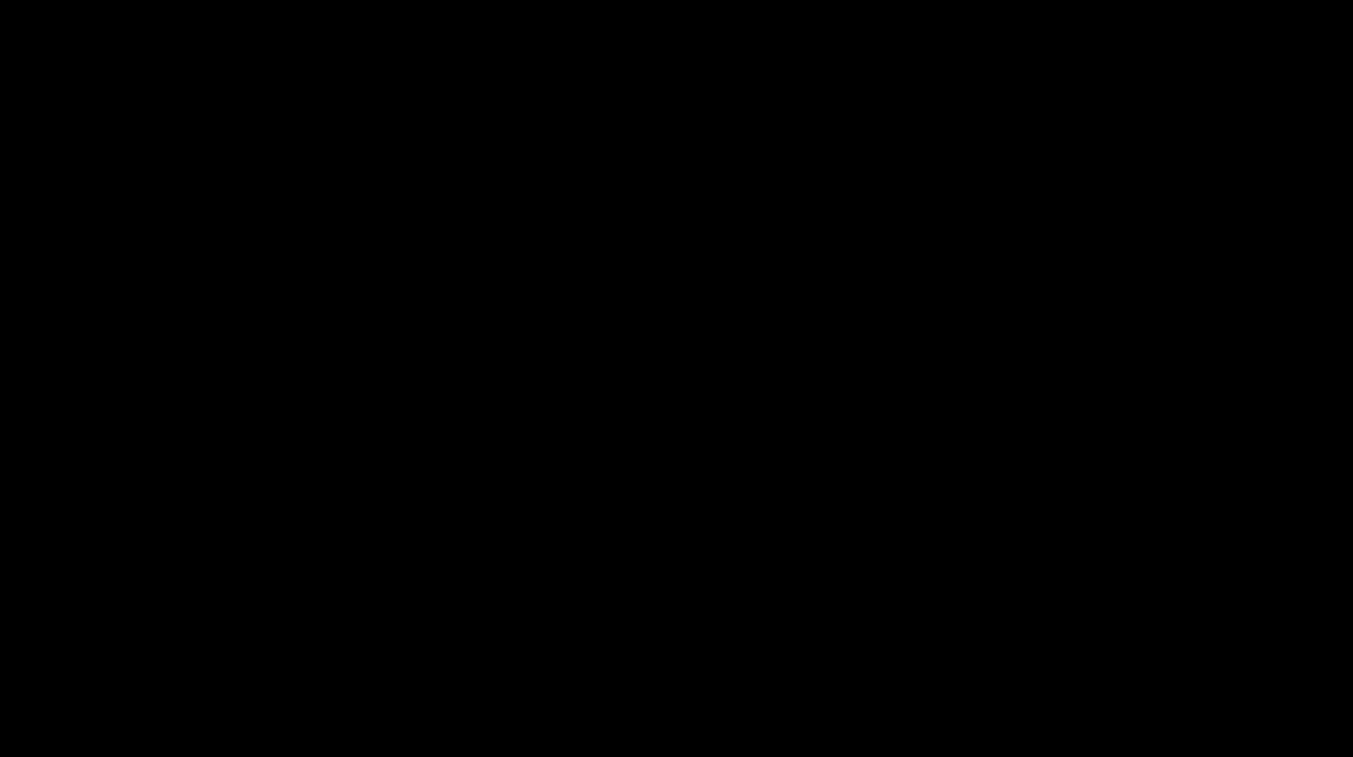
\includegraphics[width=\textwidth]{pictures/catalog.pdf} \\ 
{\tiny [174 simulations; Mroue et al; 1304.6077]}
\end{center}
  \end{column}

\end{columns}


}


\frame{
\frametitle{SpECTRE: Next-Generation Numerical Relativity}

\begin{center}

\includegraphics[width=.5\textwidth]{pictures/spectre.png} \\ 

\end{center}
\vspace{-.8cm}
\begin{columns}
  \begin{column}{.48\textwidth}
\begin{center}
    \begin{block}{\centering Science Goals}
\begin{itemize}
\scriptsize
      \item[\blacksquare]full GR
      \item[\blacksquare]neutrino-radiation-MHD
      \item[\blacksquare]temperature dependent EOS
\end{itemize}
    \end{block}
\end{center}
  \end{column}
  \begin{column}{.48\textwidth}
\begin{center}
    \begin{block}{\centering Computational Goals}
      \begin{itemize}
\scriptsize
\item[\blacksquare]Scale to O(100k) Cores
\item[\blacksquare]Discontinuous Galerkin
\item[\blacksquare]Open-Source      
      \end{itemize}
    \end{block}
\end{center}
  \end{column}

\end{columns}
\begin{tcolorbox}
\textbf{Primary Goal of PhD Thesis:} Write the SpECTRE Elliptic Solver for realistic NSNS/NSBH initial data. 
\end{tcolorbox}
{\tiny Logo From Upcoming James Bond Film}  
}

\subsection{Problems With Current Initial-Data Solvers}
\frame{
\frametitle{Problems With Current Initial-Data Solvers}

\begin{columns}
  \begin{column}{.48\textwidth}

\scriptsize The majority of NSNS simulations in the literature use polytropes or
at best, \textbf{piecewise polytropes} for stars with \textbf{low compactness} $C=M_{NS}/R_{NS} \approx .1$
\vspace{.5cm}
\begin{mybox}{white}{\centering Piecewise Polytrope}
\vspace{-.5cm}
\centering
\begin{equation*}
  P = K_{i}\rho^{\Gamma_{i}}; \,\,\,\, \rho_{i} < \rho < \rho_{i+1}
\end{equation*}
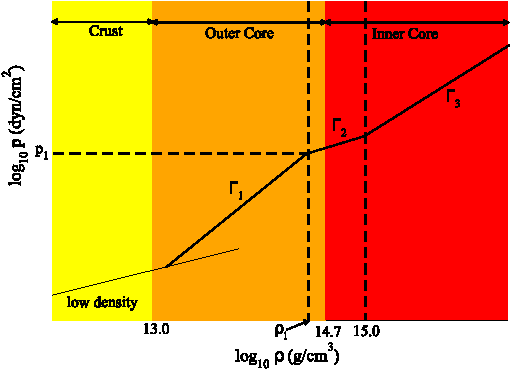
\includegraphics[width=\textwidth]{pictures/iloveq-crop.pdf}\\
\vspace{.2cm}
\centering
{\tiny [Yagi et al; 1406.7587]}
\end{mybox}
  \end{column}
  \begin{column}{.48\textwidth}
    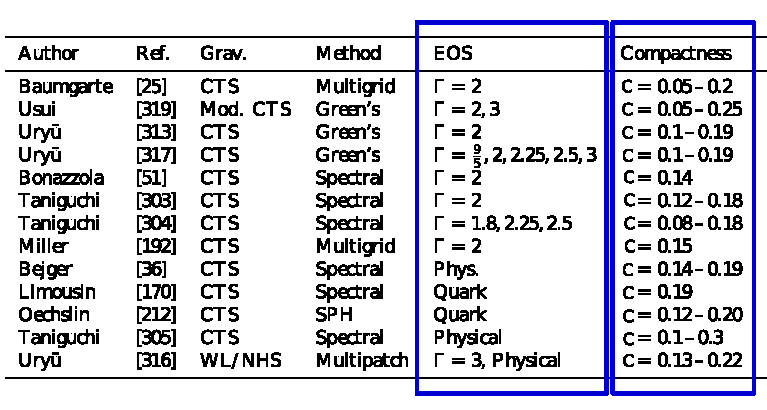
\includegraphics[width=\textwidth]{pictures/fabertable_cropped.pdf}\\
\vspace{-.2cm}
\centering{{\tiny [Faber et al; lrr-2012]}}\\
\vspace{.5cm}
\begin{tcolorbox}
\scriptsize For realistic waveform models, we need initial-data with 
\begin{itemize}
\item[\blacksquare]temperature-dependent, realistic EOS
\item[\blacksquare]any compactness
\end{itemize}

Current Solvers (SpEC, LORENE) have difficulties in this regime.
\end{tcolorbox}    
  \end{column}
\end{columns}



}



%%% Local Variables:
%%% mode: latex
%%% TeX-master: "../main"
%%% End:
